\section{Preliminary Research and Design Documentation}
\label{sec:research-design}

\subsection{Literature Review}

The project scope covers pitch book generation: taking a template, pulling financial data, planning content with an LLM, and assembling slides. RAG search over precedent materials was dropped to make room for the PowerPoint add-in (Section~\ref{sec:methodology}). The literature review focuses on what the system actually does, covering LLM productivity evidence, automated presentation generation, agentic architectures, and structured output reliability. Sources come from Google Scholar, ACM Digital Library, and IEEE Xplore, with snowball searching from \textcite{zheng2025} and \textcite{wang2024}.

\subsubsection{LLM Productivity}

Large-scale studies back up LLM productivity gains with real numbers. \textcite{brynjolfsson2023} studied 5,179 customer support agents and found a 14\% average productivity increase, with novice workers gaining up to 34\%. \textcite{noy2023} found professionals completed writing tasks 40\% faster with 18\% higher quality when using ChatGPT. Both studies show uneven benefits: less experienced workers gain most because AI gives them access to patterns that experts have already learned.

\textcite{dellacqua2023} ran a randomised experiment with 758 BCG consultants and found that those using GPT-4 completed 12.2\% more tasks, 25.1\% faster, with 40\% higher quality. Their main finding was the `jagged technological frontier': tasks inside the AI's capability boundary saw large gains, while tasks outside it made consultants perform worse. PB formatting and data retrieval sit inside the frontier. Analytical judgement sits outside it, which is why the system produces drafts rather than finished documents. \textcite{peng2023} found that developers with GitHub Copilot completed tasks 55.8\% faster, with less experienced developers benefiting most. The parallel is direct: junior analysts are the less experienced workers who stand to gain the most.

That said, none of these studies addressed template-constrained document generation where outputs must match precise visual specifications. General writing assistance helps with content but does nothing for the mechanical formatting work that consumes analyst time. This project targets that gap.

\subsubsection{Automated Presentation Generation}

Table~\ref{tab:pres-taxonomy} breaks down the main approaches to presentation generation, measured against IB requirements. Every existing approach fails on at least one dimension that IB documents require.

\begin{table}[H]
\centering
\begin{tabular}{|l|l|l|l|}
\hline
\textbf{Approach} & \textbf{Mechanism} & \textbf{Strengths} & \textbf{Limitations for IB} \\
\hline
Rule-based layout & Algorithmic text-to- & Fast, deterministic & Poor visual quality, \\
 & slide conversion & & no domain awareness \\
\hline
Rigid templates & Fixed layouts with & High visual fidelity & Cannot adapt to \\
 & manual content & & varying content lengths \\
\hline
LLM-based (PPTAgent) & Reference analysis & Preserves source & Domain-generic, \\
 & + edit-based generation & style, good content & no financial data \\
\hline
Multi-agent semantic & Template-constrained & Maintains document & Text documents only, \\
(Di Genio) & multi-agent pipeline & structure & not PowerPoint \\
\hline
VLM-based & Visual understanding & Handles complex & Approximate values, \\
 & of layouts & visual elements & not exact matching \\
\hline
\end{tabular}
\caption{Presentation Generation Approaches Compared}
\label{tab:pres-taxonomy}
\end{table}

\textcite{hu2013} introduced PPSGen, one of the first systems to learn slide generation from paper-slide pairs, but it produced rigid, text-heavy output. \textcite{yang2025} proposed Auto-Slides, a multi-agent system closer to this project's pipeline approach, but targeting academic content.

PPTAgent \parencite{zheng2025} comes closest. Its two-stage approach (analyse reference, generate matching slides) preserves the source deck's visual identity. PPTAgent outperforms earlier systems on both content and design quality. The limitation is that it targets general-purpose presentations with no financial data integration or IB narrative conventions. \textcite{liu2024} surveyed 51 professionals and found template consistency was their top priority, which backs the template-first direction. None of these tools add domain awareness.

Vision-language models offer an alternative path. \textcite{faysse2024} show VLMs can understand document layouts visually. But code-based extraction via xml2js provides exact colour hex values and font sizes, while VLM-based approaches yield approximations. For corporate template matching where a colour being off by a shade flags the document as non-compliant, exact values are non-negotiable. This is why the project uses code-based extraction over visual understanding, building on PPTAgent's template-first approach while adding the IB domain layer that PPTAgent lacks.

\subsubsection{Agentic Architectures and Tool Use}

\textcite{wang2024} propose a framework where agents operate through planning, memory, and action loops. This maps to PB generation: the system plans slide structure, remembers template constraints, and acts through tool calls and slide assembly.

\textcite{guo2024} show multi-agent systems add value when sub-tasks require negotiation or parallel reasoning. PB generation is sequential (analyse template, plan content, assemble slides), so a single agent with tool-use capabilities is sufficient. \textcite{qu2025} identify function calling as the primary LLM-tool interface, and \textcite{li2025paradigms} confirm it as the most broadly applicable pattern. In this project, the agent calls PptxGenJS to write slides and uses structured output schemas to maintain format consistency.

\subsubsection{Structured Output Reliability}

Getting reliable structured output from LLMs is a harder problem than it first appears. \textcite{shorten2024} benchmarked LLMs' ability to produce valid JSON and found an average success rate of 82.55\%, varying from 0\% to 100\% by task. \textcite{geng2025} showed that constrained decoding helps but success rates drop with schema complexity. The content plan schema in this project is moderately complex: nested slide specifications with varying content block types. These findings shaped the validation strategy: every response is validated against a Zod schema, with a fallback generic plan on failure.

\subsubsection{Hallucination and Human Oversight}

\textcite{huang2024} distinguish two types of hallucination. Intrinsic hallucination contradicts information given in the prompt. Extrinsic hallucination generates claims with no grounding in any source. For IB, extrinsic hallucination is more dangerous: made-up numbers or invented deal precedents could reach clients and regulators, causing regulatory problems or legal liability.

\textcite{alansari2025} group prevention into three categories: grounding outputs in real sources, forcing structured output formats, and human review. No single strategy eliminates hallucination. This project layers all three: financial data comes from APIs rather than LLM generation, structured JSON schemas enforce the format of each slide specification, and human review is mandatory before any output reaches a client.

\textcite{wu2022} classify HITL approaches into data processing, interventional training, and system design. This project uses system design: the analyst defines inputs, reviews outputs, and decides whether to use them. The EU AI Act requires human oversight for AI in financial services \parencite{bis2024}, making this a compliance requirement as well as a design choice. Junior analysts already produce drafts that senior bankers revise. The system replaces the blank page, not the review process.

\subsubsection{Research Gaps}

Four gaps emerge from this review. First, no presentation generation tool targets IB-specific conventions. PPTAgent \parencite{zheng2025}, Auto-Slides \parencite{yang2025}, and PPSGen \parencite{hu2013} all target general or academic presentations. Second, no system automates both structure and content within a single pipeline \parencite{achachlouei2023}. Third, no system integrates data retrieval with template-aware assembly. Fourth, the productivity literature measures general tasks but none measured template-constrained document generation where outputs must match precise visual specifications.

This project targets these gaps with code-based template extraction for exact visual matching, IB-specific content planning, and mandatory human review for accuracy. The evaluation measures template matching and generation speed, and includes an informal usability evaluation with junior analysts.

\subsection{System Design}

This section documents the system architecture, data models, and component specifications derived from the requirements and literature review. The design puts template matching, clean separation of components, and human oversight first.

\subsubsection{Architecture Overview}

Figure~\ref{fig:architecture} shows the high-level system architecture. The design follows a pipeline pattern with three main stages: template analysis, content planning, and slide assembly.

\begin{figure}[H]
\centering
\begin{tikzpicture}[
    node distance=2cm and 4cm,
    box/.style={draw, rounded corners, minimum width=3.5cm, minimum height=1.1cm, align=center, font=\small},
    data/.style={draw, dashed, rounded corners, minimum width=3cm, minimum height=0.9cm, align=center, font=\footnotesize},
    arr/.style={->, thick, >=stealth}
]
% Main column
\node[data] (input) {User Input\\(company, template, type)};
\node[box, below=of input] (ta) {Template Analyser};
\node[box, below=of ta] (cp) {Content Planner\\(LLM Agent)};
\node[box, below=of cp] (sb) {Slide Builder};
\node[data, below=of sb] (out) {Generated PB (.pptx)};
\node[box, below=1.2cm of out] (hr) {Human Review};

% Side nodes
\node[data, left=of ta] (ref) {Reference\\Template (.pptx)};
\node[data, right=of cp] (dr) {Data Retrieval\\(stretch goal)};

% Arrows - main flow
\draw[arr] (input) -- (ta);
\draw[arr] (ta) -- (cp);
\draw[arr] (cp) -- (sb);
\draw[arr] (sb) -- (out);
\draw[arr] (out) -- (hr);

% Side arrows
\draw[arr] (ref) -- (ta);
\draw[arr, dashed] (dr) -- (cp);

% Content Plan on the left, between planner and builder
\node[data, left=of sb] (plan) {Content\\Plan (JSON)};
\draw[arr] (cp.west) -- ++(-1.8,0) |- (plan.north);
\draw[arr] (plan.east) -- (sb.west);
\end{tikzpicture}
\caption{System Architecture showing the three-stage core pipeline. Data Retrieval is a stretch goal.}
\label{fig:architecture}
\end{figure}

The architecture separates concerns into independent modules (SE2, SE9). The Template Analyser extracts layout patterns without generating content. The Content Planner uses an LLM to structure the narrative without touching PowerPoint files. The Slide Builder assembles files from specifications without making content decisions. This separation supports testing and allows components to be reused independently. Data Retrieval from external APIs is a stretch goal that can be added later without changing the core pipeline.

\newpage
\subsubsection{Data Models}

The system uses two primary data structures that flow between components. Table~\ref{tab:data-models} lists the fields.

\begin{table}[H]
\centering
\begin{tabular}{|l|l|l|}
\hline
\textbf{Model} & \textbf{Key Fields} & \textbf{Purpose} \\
\hline
TemplateSchema & layouts[], colours, fonts, & Stores extracted template properties \\
 & placeholders[] & for content planning and slide assembly \\
\hline
SlideLayout & layout\_index, placeholder\_map, & Maps placeholder positions to \\
 & background & content types for a single layout \\
\hline
ContentPlan & slides[], metadata & LLM-generated specification of \\
 & & slide content and structure \\
\hline
SlideSpec & layout\_id, placeholders, & Content specification for \\
 & charts[], tables[] & a single slide \\
\hline
\end{tabular}
\caption{Primary Data Model Specifications}
\label{tab:data-models}
\end{table}

\textbf{Template Schema} captures extracted template properties including layouts, colour palettes, fonts, and placeholder specifications. Each slide layout maps placeholder indices to content types (title, body, picture, chart, table).

\textbf{Content Plan} specifies the content for each slide: which layout to use, what text goes in each placeholder, and what data to display. The LLM generates this structure. The Slide Builder consumes it.

\newpage

Figure~\ref{fig:er-diagram} shows the database schema. Row-level security (RLS) policies on every table restrict access so that authenticated users can only read and write their own records.

\begin{figure}[H]
\centering
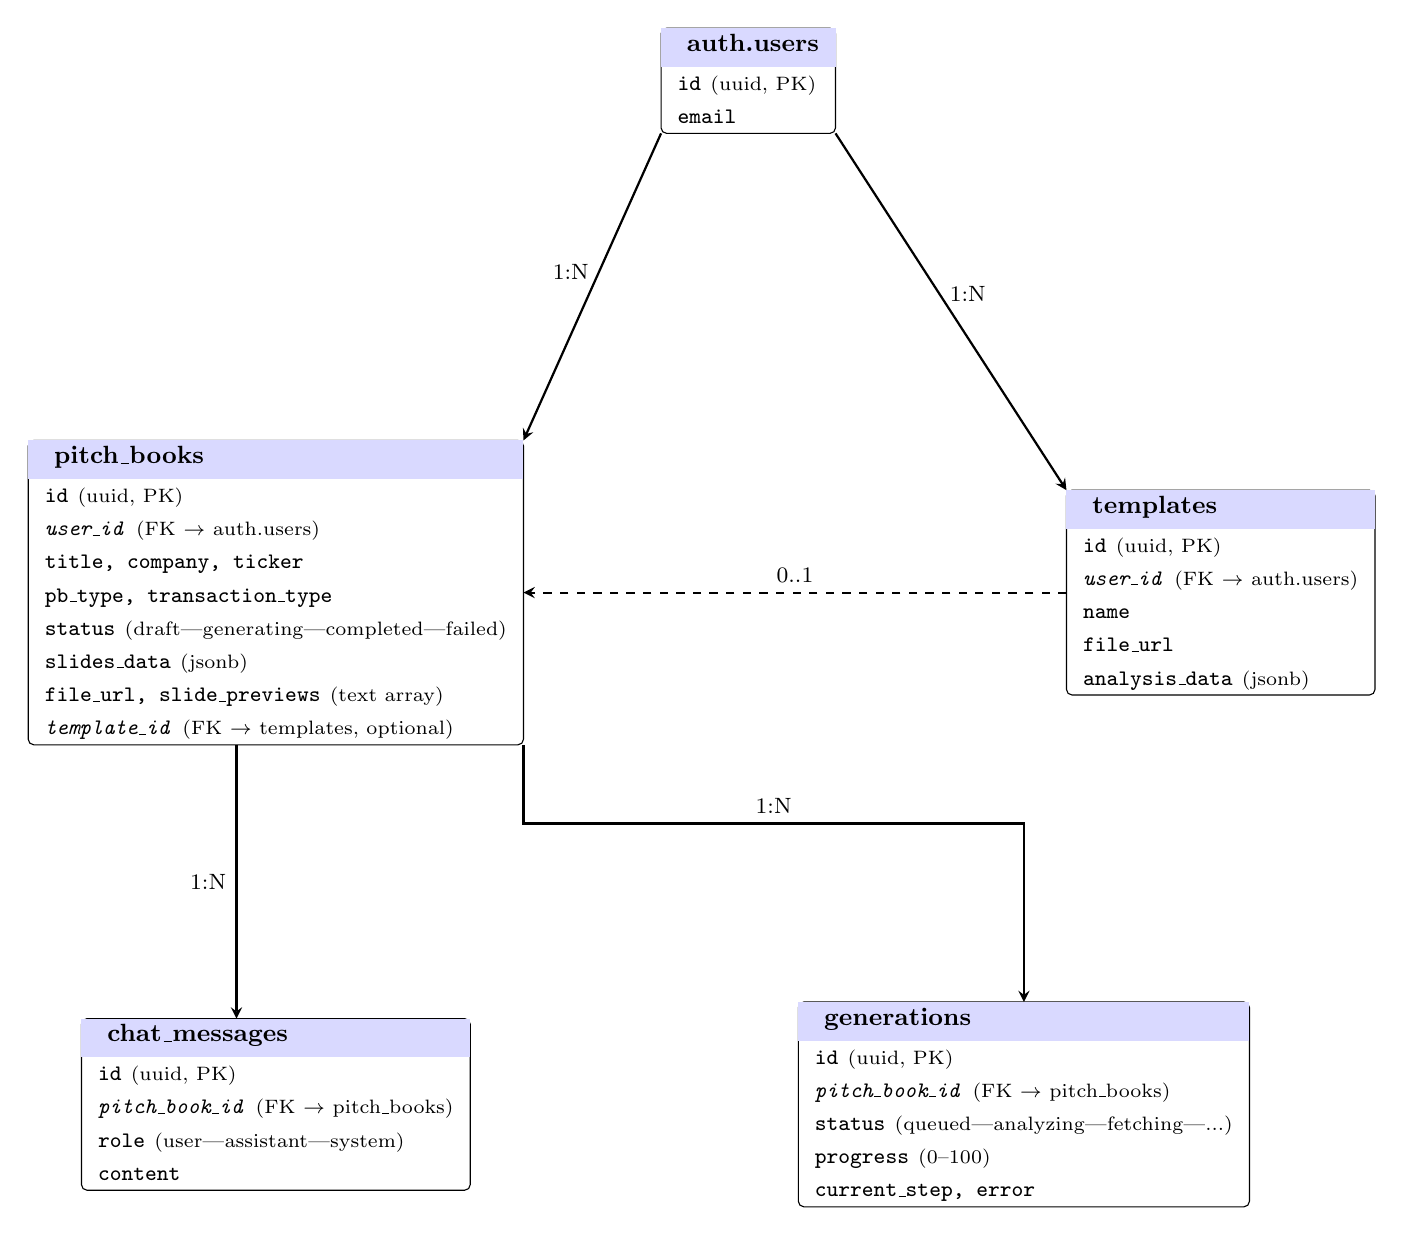
\begin{tikzpicture}[
    table/.style={draw, rectangle, rounded corners=2pt, inner sep=0pt, outer sep=0pt},
    rel/.style={->, thick, >=stealth},
]

% ── auth.users ──
\node[table] (users) at (6, 14) {
  \begin{tabular}{l}
    \cellcolor{blue!15} \textbf{\small auth.users} \\[2pt]
    \textbf{\footnotesize\ttfamily id} \textnormal{\scriptsize (uuid, PK)} \\
    {\footnotesize\ttfamily email} \\
  \end{tabular}
};

% ── pitch_books ──
\node[table] (pb) at (0, 7.5) {
  \begin{tabular}{l}
    \cellcolor{blue!15} \textbf{\small pitch\_books} \\[2pt]
    \textbf{\footnotesize\ttfamily id} \textnormal{\scriptsize (uuid, PK)} \\
    \textit{\footnotesize\ttfamily user\_id} \textnormal{\scriptsize (FK $\to$ auth.users)} \\
    {\footnotesize\ttfamily title, company, ticker} \\
    {\footnotesize\ttfamily pb\_type, transaction\_type} \\
    {\footnotesize\ttfamily status} \textnormal{\scriptsize (draft|generating|completed|failed)} \\
    {\footnotesize\ttfamily slides\_data} \textnormal{\scriptsize (jsonb)} \\
    {\footnotesize\ttfamily file\_url, slide\_previews} \textnormal{\scriptsize (text array)} \\
    \textit{\footnotesize\ttfamily template\_id} \textnormal{\scriptsize (FK $\to$ templates, optional)} \\
  \end{tabular}
};

% ── templates ──
\node[table] (tmpl) at (12, 7.5) {
  \begin{tabular}{l}
    \cellcolor{blue!15} \textbf{\small templates} \\[2pt]
    \textbf{\footnotesize\ttfamily id} \textnormal{\scriptsize (uuid, PK)} \\
    \textit{\footnotesize\ttfamily user\_id} \textnormal{\scriptsize (FK $\to$ auth.users)} \\
    {\footnotesize\ttfamily name} \\
    {\footnotesize\ttfamily file\_url} \\
    {\footnotesize\ttfamily analysis\_data} \textnormal{\scriptsize (jsonb)} \\
  \end{tabular}
};

% ── chat_messages ──
\node[table] (chat) at (0, 1) {
  \begin{tabular}{l}
    \cellcolor{blue!15} \textbf{\small chat\_messages} \\[2pt]
    \textbf{\footnotesize\ttfamily id} \textnormal{\scriptsize (uuid, PK)} \\
    \textit{\footnotesize\ttfamily pitch\_book\_id} \textnormal{\scriptsize (FK $\to$ pitch\_books)} \\
    {\footnotesize\ttfamily role} \textnormal{\scriptsize (user|assistant|system)} \\
    {\footnotesize\ttfamily content} \\
  \end{tabular}
};

% ── generations ──
\node[table] (gen) at (9.5, 1) {
  \begin{tabular}{l}
    \cellcolor{blue!15} \textbf{\small generations} \\[2pt]
    \textbf{\footnotesize\ttfamily id} \textnormal{\scriptsize (uuid, PK)} \\
    \textit{\footnotesize\ttfamily pitch\_book\_id} \textnormal{\scriptsize (FK $\to$ pitch\_books)} \\
    {\footnotesize\ttfamily status} \textnormal{\scriptsize (queued|analyzing|fetching|...)} \\
    {\footnotesize\ttfamily progress} \textnormal{\scriptsize (0--100)} \\
    {\footnotesize\ttfamily current\_step, error} \\
  \end{tabular}
};

% ── Relationships (routed to avoid overlaps) ──
% users -> pitch_books
\draw[rel] (users.south west) -- node[left, font=\footnotesize, pos=0.45] {1:N} (pb.north east);
% users -> templates
\draw[rel] (users.south east) -- node[right, font=\footnotesize, pos=0.45] {1:N} (tmpl.north west);
% pitch_books -> chat_messages (straight down, left side)
\draw[rel] ([xshift=-0.5cm]pb.south) -- node[left, font=\footnotesize, pos=0.5] {1:N} ([xshift=-0.5cm]chat.north);
% pitch_books -> generations (route right then down to avoid overlap)
\draw[rel] (pb.south east) -- ++(0,-1) -| node[above, font=\footnotesize, pos=0.25] {1:N} (gen.north);
% templates -..-> pitch_books (optional FK, horizontal)
\draw[rel, dashed] (tmpl.west) -- node[above, font=\footnotesize] {0..1} (pb.east);

\end{tikzpicture}%
}
\caption{Database entity-relationship diagram. Primary keys in bold, foreign keys in italics. All tables use UUID primary keys with row-level security. The dashed line indicates an optional foreign key (pitch books may or may not reference a template).}
\label{fig:er-diagram}
\end{figure}

\subsubsection{Component Specifications}

\textbf{Template Analyser.} Input: reference .pptx file. Output: TemplateSchema JSON. Uses JSZip and xml2js to parse the .pptx file at the XML level, extracting slide masters, layouts, colour schemes, and placeholder positions. Identifies placeholder types (title, body, picture, chart, table) by inspecting shape properties. Extracts exact colour values as hex codes and font specifications including family, size, and weight.

\textbf{Content Planner.} Input: user parameters, TemplateSchema. Output: ContentPlan JSON. Implemented as an LLM call with JSON schema validation to check the output structure. Selects appropriate layouts from the template schema based on content requirements. Plans slide sequence following IB narrative conventions (context, analysis, recommendation).

\textbf{Slide Builder.} Input: ContentPlan, TemplateSchema, reference template. Output: .pptx file. Uses PptxGenJS to generate slides with code. Iterates through ContentPlan slides, selects layouts, and populates placeholders. Applies exact formatting from TemplateSchema. Generates charts and tables with code.

\subsubsection{API Design}

The backend exposes a REST API via Express.js. The primary endpoint accepts generation requests and returns job identifiers for async processing.

\vspace{0.5em}\filbreak
\begin{lstlisting}[language=JavaScript, caption=Pitch book creation request interface (from shared-types)]
// POST /api/pitchbooks - returns pitch book record with generation queued
interface CreatePitchBookRequest {
  title: string;
  company: string;
  ticker?: string;
  transaction_type: 'ma' | 'capital_raising' | 'restructuring'
                    | 'ipo' | 'debt_financing';
  pb_type: 'company_overview' | 'market_update'
           | 'transaction_summary';
  template_id?: string;       // reference template UUID
  additional_context?: string; // free-text instructions
  color_theme?: string;        // e.g. 'navy_gold', 'teal_coral'
  design_style?: string;
}
\end{lstlisting}

The full API is documented with an OpenAPI 3.0 specification and served through Swagger UI (Figure~\ref{fig:swagger}). Authenticated endpoints (marked with a lock icon) require a valid Supabase session cookie.

\begin{figure}[H]
\centering
\screenshot{screenshots/deployment/swagger.png}
\caption{Swagger UI showing the REST API endpoints grouped by resource: Companies (data retrieval), Pitch Books (generation and CRUD), and Templates (upload and analysis).}
\label{fig:swagger}
\end{figure}

\subsubsection{Design Trade-offs}

Table~\ref{tab:tradeoffs} summarises the four main design trade-offs.

\begin{table}[H]
\centering
\begin{tabular}{|l|l|l|}
\hline
\textbf{Decision} & \textbf{Chosen Option} & \textbf{Rationale} \\
\hline
Single vs multi-agent & Single agent with tools & PB generation is sequential; \\
 & & multi-agent overhead not justified \\
\hline
Programmatic vs VLM & Programmatic extraction & Exact values needed for \\
template extraction & (JSZip + xml2js) & corporate template matching \\
\hline
SDK vs custom & Structured LLM calls & Vendor-agnostic; component \\
orchestration & with JSON schemas & interfaces allow swapping later \\
\hline
Sync vs async & Async job processing & Generation takes minutes; \\
generation & & users poll for completion \\
\hline
\end{tabular}
\caption{Design Trade-offs}
\label{tab:tradeoffs}
\end{table}

\subsubsection{Data Flow}

Figure~\ref{fig:dataflow} shows how data moves through the system during a generation request.

\begin{figure}[H]
\centering
\begin{tikzpicture}[
    node distance=2.2cm and 2cm,
    box/.style={draw, rounded corners, minimum width=3.2cm, minimum height=1cm, align=center},
    data/.style={draw, dashed, rounded corners, minimum width=2.8cm, minimum height=0.8cm, align=center, font=\small},
    arr/.style={->, thick, >=stealth}
]
% Main pipeline down the centre
\node[box] (iv) {Input Validation};
\node[box, below=of iv] (te) {Template Extraction};
\node[box, below=of te] (cpl) {Content Planning};
\node[box, below=of cpl] (sa) {Slide Assembly};
\node[data, below=1.5cm of sa] (out) {Generated .pptx};

% Inputs above validation, spread apart
\node[data, above=1.2cm of iv, xshift=-2.5cm] (t) {.pptx Template};
\node[data, above=1.2cm of iv, xshift=2.5cm] (u) {User Parameters};

% Side data stores - simple left-side placement
\node[data, left=3cm of te, yshift=-1.1cm] (ts) {Template\\Schema};
\node[data, left=3cm of cpl, yshift=-1.1cm] (cp) {Content\\Plan};

% Input arrows into validation
\draw[arr] (t.south) -- ([xshift=-0.8cm]iv.north);
\draw[arr] (u.south) -- ([xshift=0.8cm]iv.north);

% Main flow
\draw[arr] (iv) -- (te);
\draw[arr] (te) -- (cpl);
\draw[arr] (cpl) -- (sa);
\draw[arr] (sa) -- (out);

% Template Schema: extraction produces, planning consumes
\draw[arr] (te.south west) -- (ts.north east);
\draw[arr] (ts.south east) -- (cpl.north west);

% Content Plan: planning produces, assembly consumes
\draw[arr] (cpl.south west) -- (cp.north east);
\draw[arr] (cp.south east) -- (sa.north west);
\end{tikzpicture}
\caption{Data flow through the generation pipeline}
\label{fig:dataflow}
\end{figure}

\subsubsection{Design Limitations}

The system cannot generate charts from scratch. It can only populate existing chart placeholders. The template analyser handles standard placeholder-based layouts but does not reverse-engineer arbitrary PowerPoint constructions with overlapping elements or custom animations. The content planner has no memory across sessions. The system produces drafts, not finished documents: human review is mandatory (K6, SE1).
